\section{Quantum Signal Processing}
\label{sec:preliminaries}

The essential mechanism of quantum signal processing is
visible in Grover's search
algorithm~\cite{Grover1997}.  There, the quantum state
evolves within a two-dimensional subspace spanned by
the initial superposition $\ket{\psi_0}$ and the target
state $\ket{\psi_*}$.  Two operations alternate: an
oracle reflection
$U_f = I - 2\ket{\psi_*}\!\bra{\psi_*}$ that flips
the sign of the target component, and a diffusion
operator $D = 2\ket{\psi_0}\!\bra{\psi_0} - I$ that
reflects about the initial state.  Because two
reflections in a plane compose to a rotation, each
Grover iteration rotates the state by a fixed angle
$2\theta$, where
$\sin\theta = \langle\psi_*|\psi_0\rangle$ is the
overlap with the target
(Fig.~\ref{fig:grover-qsp};
see also Ref.~\cite{BenentiCasatiStrini2004}, Fig.~3.24).  The initial state
already makes an angle $\theta$ with the
non-target axis, so after $k$ iterations the amplitude
on the target is $\sin\!\big((2k{+}1)\theta\big)$---a
trigonometric polynomial of the signal
$a = \cos\theta$.

\begin{figure}[t]
	\centering
	%% Panel (a): Matplotlib Bloch-sphere figure
	\begin{minipage}{\columnwidth}
		\raggedright
		\hspace{0.2em}\textbf{(a)}\\[-2pt]
		\centering
		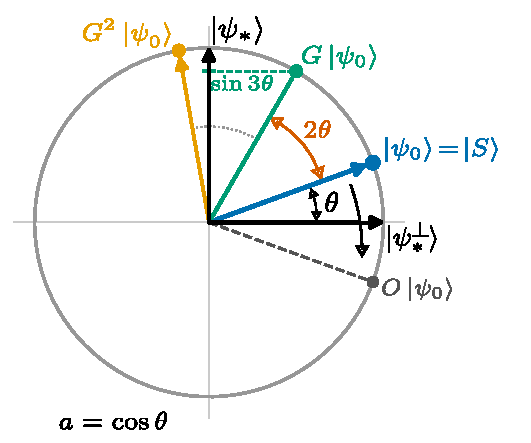
\includegraphics[width=0.75\columnwidth]{figures/grover_bloch.pdf}
	\end{minipage}\\[6pt]
	%% Panel (b): QSP circuit (quantikz)
	\begin{minipage}{\columnwidth}
		\raggedright
		\hspace{0.2em}\textbf{(b)}\\[-2pt]
		\centering
	\end{minipage}\\[-2pt]
	\begin{quantikz}[column sep=0.15cm, row sep=0.3cm]
		\lstick{\footnotesize$\ket{0}$}
		& \gate{\phi_0}
		& \gate{W}
		& \gate{\phi_1}
		& \gate{W}
		& \ \cdots\ \qw
		& \gate{W}
		& \gate{\phi_d}
		& \qw
	\end{quantikz}
	\caption{%
		Geometric picture of quantum signal processing.
		\textbf{(a)}~Grover's algorithm in the two-dimensional
		plane spanned by the target state $\ket{\psi_*}$ and its
		complement $\ket{\psi_*^{\perp}}$.  The initial
		superposition $\ket{\psi_0} = \ket{S}$ lies at angle
		$\theta$ from $\ket{\psi_*^{\perp}}$, where
		$\sin\theta = \langle \psi_* | \psi_0 \rangle$.  The oracle
		reflects about $\ket{\psi_*^{\perp}}$ (dashed), and
		the combined Grover operator $G$ rotates by $2\theta$
		toward the target; after $k$ iterations the target-state
		amplitude is $\sin\!\big((2k{+}1)\theta\big)$---a
		trigonometric polynomial of the signal
		$a = \cos\theta$.  The dashed projection shows $\sin 3\theta$
		after one iteration.
		\textbf{(b)}~The QSP circuit generalizes this structure:
		signal rotations $W(a)$ alternate with tunable phase gates
		$\exp[i\phi_j \PauliZ]$.  In Grover's algorithm all phases are
		equal; in QSP they are free parameters that produce
		arbitrary bounded polynomials of~$a$.}
	\label{fig:grover-qsp}
\end{figure}

This geometric picture reveals the core structure of
quantum signal
processing~\cite{LowChuang2017,GSLW2019}: an
alternating sequence of signal-dependent rotations and
tunable control operations, acting in a two-dimensional
subspace, whose amplitudes are polynomial functions of
the bounded parameter $a = \cos\theta \in [-1,1]$.
Where Grover uses equal rotation angles at every step
and produces a single trigonometric polynomial, QSP
allows the control rotations to vary independently,
thereby accessing arbitrary polynomial transformations
of~$a$.  (The precise sense in which Grover's algorithm
is a special case of QSP---through product-formula
approximation of imaginary-time evolution on the
unitary group---has been established by Suzuki
et~al.~\cite{SuzukiEtAl2025}.)

Concretely, define the signal unitary for a bounded
value $a \in [-1,1]$:
\begin{equation}
	W(a) = \begin{pmatrix} a             & i\sqrt{1-a^2} \\
                i\sqrt{1-a^2} & a\end{pmatrix},
	\label{eq:standard-signal}
\end{equation}
a rotation by $\arccos(a)$ in the $xz$-plane of the
Bloch sphere.  A QSP sequence interleaves $d$
applications of $W(a)$ with $d+1$ tunable phase gates
$\exp[i\phi_j\PauliZ]$, producing the unitary
\begin{equation}
	U_{\bm{\phi}}(a)
	= \exp[i\phi_0\PauliZ]
	\prod_{j=1}^{d} W(a)\,\exp[i\phi_j\PauliZ],
	\label{eq:standard-qsp}
\end{equation}
where $\bm{\phi} = (\phi_0, \ldots, \phi_d) \in \R^{d+1}$
are the phase angles.  Setting all phases equal recovers
Grover's algorithm; allowing them to vary independently
gives access to a much larger family of polynomial
transformations of~$a$.

Which polynomial transformations of~$a$ can be realized
by choosing the phases~$\bm{\phi}$?  Unitarity imposes
an immediate constraint: the matrix element
$P(a) = \bra{0}U_{\bm{\phi}}(a)\ket{0}$ satisfies
$|P(a)| \leq 1$ for all $a \in [-1,1]$, since
$|\!\bra{0}U\ket{0}\!| \leq 1$ for any unitary~$U$.
The QSP theorem establishes that this boundedness
condition, together with a parity constraint inherited
from the signal unitary, is also sufficient.

\begin{theorem}[QSP Theorem~\cite{GSLW2019}]
	\label{thm:standard-qsp}
	For every polynomial $P: [-1,1] \to \C$ of degree at
	most $d$ satisfying
	\begin{enumerate}
		\item $|P(a)| \leq 1$ for all $a \in [-1,1]$,
		\item $P$ has definite parity: $P(-a) = \pm P(a)$,
	\end{enumerate}
	there exist phase angles $\bm{\phi}$ such that
	$\bra{0}U_{\bm{\phi}}(a)\ket{0} = P(a)$.
\end{theorem}

Theorem~\ref{thm:standard-qsp} is a completeness
result: every bounded polynomial of definite parity is
achievable, and efficient algorithms exist for
computing the required
phases~\cite{DongMengWhaleyEtAl2021,Haah2019}.
It also determines the full output state.  Because
$U_{\bm{\phi}}$ is unitary, its action on $\ket{0}$
must produce a normalized two-component state:
\begin{equation}
	U_{\bm{\phi}}(a)\ket{0}
	= P(a)\ket{0} + Q(a)\sqrt{1-a^2}\,\ket{1},
	\label{eq:qsp-output-state}
\end{equation}
where $Q(a)$ is a complementary polynomial of degree
at most~$d-1$ and opposite parity, constrained by
$|P(a)|^2 + (1-a^2)|Q(a)|^2 = 1$.  Both components
are therefore bounded by~$1$ in absolute value.

Chebyshev polynomials enter for the same reason they
appear in Grover's algorithm.  Writing
$a = \cos\theta$, the signal unitary becomes a rotation
by~$\theta$, and its $k$-fold application gives
$W^k\ket{0} = \cos(k\theta)\ket{0} +
	i\sin(k\theta)\ket{1}$.  The Chebyshev polynomials of
the first and second kind,
\begin{align}
	T_k(\cos\theta)     & = \cos(k\theta),
	\label{eq:cheby-T-def}                                    \\
	U_{k-1}(\cos\theta) & = \frac{\sin(k\theta)}{\sin\theta},
	\label{eq:cheby-U-def}
\end{align}
are therefore the natural basis: the
$\ket{0}$-amplitude after $k$ signal applications is
$\bra{0}W^k\ket{0} = T_k(a)$, the Chebyshev
polynomial already visible in Grover's algorithm.
These functions form a complete orthogonal set on
$[-1,1]$ with weight $(1-x^2)^{-1/2}$, and every QSP
polynomial is a finite Chebyshev expansion whose
coefficients are determined by the phase
angles~$\bm{\phi}$.  Grover's algorithm activates only
a single term; QSP, by varying the phases
independently, can populate the entire basis.

Yet this expressiveness is limited by the very
constraint that enables it: $|P(a)| \leq 1$.  In the
principal application---eigenvalue
transformation---the signal is
$a = \lambda/\alpha$, where $\lambda$ is an eigenvalue
of a Hermitian operator~$H$ and
$\alpha \geq \|H\|$ is a normalization factor chosen
so that $a \in [-1,1]$.  The block encoding
framework~\cite{GSLW2019} embeds $H$ into a larger
unitary so that $a$ appears as the signal in each
eigenspace, and QSP then implements the polynomial
transformation $P(\lambda/\alpha)$ of each eigenvalue.
The boundedness constraint $|P| \leq 1$ carries three
concrete costs: it requires knowledge of~$\|H\|$ (or
an upper bound) to fix the normalization; it inflates
circuit depth by a factor of~$\alpha$, since each
query acts on the rescaled operator $H/\alpha$; and it
excludes unbounded target functions---$1/\lambda$,
$\lambda$, $\tan(\lambda)$---that cannot be
approximated by polynomials bounded on $[-1,1]$
without truncation and regularization.  All three
costs share the same origin: the signal must satisfy
$|a| \leq 1$ because the standard encoding writes it
into a state amplitude.  If data could be placed on
the Bloch sphere without this restriction, the
boundedness constraint would never arise.  The next
section shows that stereographic projection provides
exactly such an encoding.
